
%\clearpage

%\section{Introduction}  % =========================================================================

%TODO

\clearpage

\section{WrightTools}  % =============================================================

This section was originally published in the Journal of Open Source Software \cite{ThompsonBlaiseJonathan2019a}.

\hypertarget{introduction}{%
\subsection{Introduction}\label{introduction}}

``Multidimensional spectroscopy'' (MDS) is a family of analytical
techniques that record the response of a material to multiple
stimuli---typically multiple ultrafast pulses of light. This approach
has several unique capabilities:

\begin{itemize}
\item
	resolving congested states \cite{ZhaoWei1999b}\cite{DonaldsonPaulMurray2008a},
\item
  extracting spectra that would otherwise be selection-rule disallowed
		\cite{BoyleErinSelene2013b}\cite{BoyleErinSelene2014a},
\item
  resolving fully coherent dynamics \cite{PakoulevAndreiV2009a},
\item
  measuring coupling \cite{WrightJohnCurtis2011a},
\item
	and resolving ultrafast dynamics \cite{SmallwoodChristopherL2018a}\cite{CzechKyleJonathan2015a}.
\end{itemize}

In our view, the most exciting aspect of these techniques is the vast
number of different approaches that scientists can take to learn about
material quantum states. Often, a number of these experiments can be
accomplished with a single instrument. The diversity of
related-but-unique approaches to interrogating quantum systems is an
important strength of MDS.

Advancements in optics and laser science are bringing ultrafast
multidimensional spectroscopy to more and more laboratories around the
world. At the same time, increasing automation and computer control are
allowing traditionally ``one-dimensional'' spectroscopies to be recorded
against other dimensions.

Due to its diversity and dimensionality, MDS data is challenging to
process and visualize. The tools that scientists develop to process one
experiment may not work when different experimental variables are
explored. Historically, MDS practitioners have developed custom, one-off
data processing workflows that need to be radically changed when new
experiments are undertaken. These changes take time to implement, and
can become annoyances or opportunities for error. Even worse, the
challenge of designing a new processing workflow may dissuade a
scientist from creatively modifying their experimental strategy, or
comparing their data with data taken from another instrument. This limit
to creativity and flexibility defeats one of the main advantages of the
MDS ``family approach''.

\texttt{WrightTools} is a new Python package that is made specifically
for multidimensional spectroscopy. It aims to be a core toolkit that is
general enough to handle all MDS datasets and processing workloads.
Being built for and by MDS practitioners, \texttt{WrightTools} has an
intuitive, high-level, object-oriented interface for spectroscopists. To
our knowledge, \texttt{WrightTools} is the first MDS-focused toolkit to
be freely avaliable and openly licensed.

\hypertarget{challenges-and-implementation}{%
\subsection{Challenges and
Implementation}\label{challenges-and-implementation}}

There are several recurring challenges in MDS data processing and
representation:

\begin{itemize}
\item
  There are no agreed-upon file formats. Files generated by researchers
  may have inconsistent internal conventions, and they often fail to be
  fully self-describing.
\item
  There is a great diversity of dataset types. The same instrument is
  capable of producing datasets with many different combinations of
  scanned hardware.
\item
  Dataset size may be large enough to run into computer memory limits.
\item
  Dataset dimensionality is large enough to represent challenges in
  human interaction and visualization.
\end{itemize}

The excellent Scientific Python ecosystem is well suited to address all
of these challenges \cite{OliphantTravisE2007a}. Numpy supports
interaction with and manipulation of multidimensional arrays
\cite{OliphantTravisE2006a}. Matplotlib supports one, two, and even
three-dimensional plotting \cite{HunterJohnD2007a}. h5py
\cite{ColletteAndrew2013} interfaces with hdf5 \cite{hdf5}, allowing for
storage and memory-safe access to large multidimensional arrays in a
binary format that can be accessed from a variety of different popular
languages, including MATLAB and Fortran. \texttt{WrightTools} does not
intend to replace or reimplement these core libraries. Instead,
\texttt{WrightTools} offers an interface that impedance-matches
multidimensional spectroscopy and Scientific Python.

\texttt{WrightTools} defines a universal MDS data format: the
\texttt{wt5} file. These are simply hdf5 files with certain internal
conventions that are designed for MDS. These internal conventions enable
the flexibility and ease-of-use that we discuss in the rest of this
section. Instances of WrightTools's classes dynamically interact with
the multidimensional spectroscopic data within these files. These
classes are children of h5py classes. \texttt{WrightTools} offers a
variety of functions that try hard to convert data stored in various
other formats to \texttt{wt5}.

\texttt{WrightTools} defines a unique and flexable strategy of storing
and manipulating MDS datasets. A single instance of the
\texttt{WrightTools.Data} class is implemented as a group containing
many separate arrays. There are two principle multidimensional array
classes: \texttt{Channel} and \texttt{Variable}. Conceptually, these
correspond to independent (scanned) dimensions---``variables''---and
dependent (measured) signals---``channels''. Channels typically contain
measured signals from all of the different sensors that are employed
simultaneously during a MDS experiment. Variables contain coordinates of
different light manipulation hardware that are scanned against
each-other to make up an MDS experiment. All variables are recorded,
including coordinates for hardware that are not actually moved during
that experiment (an array with one unique value) or other independent
variables, such as lab time.

There can be many variables that change in the context of a single MDS
experiment. The typical spectroscopist only really cares about a small
subset of these variables, but exactly what subset matters may change as
different strategies are used to explore the dataset. Furthermore, it is
often useful to ``combine'' multiple variables using simple algebraic
relationships to exploit the natural symmetry of many MDS experiments
and to draw comparisons between different members of the MDS family
\cite{NeffMallonNathanA2017a}. In light of these details,
\texttt{WrightTools} provides a high-level \texttt{Axis} class that
allows users to transparently define which variables, variable
relationships, and unit conventions are important to them for
representation and manipulation. Each \texttt{Axis} contains an
\texttt{expression}, which dictates its relationship with one or more
variables. Given 5 variables with names
{[}\texttt{\textquotesingle{}w1\textquotesingle{}},
\texttt{\textquotesingle{}w2\textquotesingle{}},
\texttt{\textquotesingle{}wm\textquotesingle{}},
\texttt{\textquotesingle{}d1\textquotesingle{}},
\texttt{\textquotesingle{}d2\textquotesingle{}}{]} , example valid
expressions include \texttt{\textquotesingle{}w1\textquotesingle{}},
\texttt{\textquotesingle{}w1=wm\textquotesingle{}},
\texttt{\textquotesingle{}w1+w2\textquotesingle{}},
\texttt{\textquotesingle{}2*w1\textquotesingle{}},
\texttt{\textquotesingle{}d1-d2\textquotesingle{}}, and
\texttt{\textquotesingle{}wm-w1+w2\textquotesingle{}}. Users may treat
axes like multidimensional arrays, using \texttt{\_\_getitem\_\_} syntax
and slicing, but axes do not themselves contain arrays. Instead, the
appropriate axis value at each dataset coordinate is computed on-the-fly
using the given expression. Users may at any time change their axes by
simply calling \texttt{transform} with new expressions.

\texttt{WrightTools} offers a suite of data manipulation tools with MDS
in mind. Users can access portions of their data using high-level
methods like \texttt{chop}, \texttt{split}, and \texttt{clip}. They can
process their data using simple mathematical operations or more specific
tools like \texttt{level}, \texttt{gradient}, \texttt{collapse}, and
\texttt{smooth}. Users can even \texttt{join} multiple datasets
together, creating higher-dimensional datasets when appropriate. All of
these operations refer to the self-describing internal structure of the
\texttt{wt5} file wherever possible. Users are not asked to refer to the
specific shape and indicies of their data arrays. Instead, they deal
with simple axis expressions and unit-aware coordinates.

\texttt{WrightTools} offers a set of ``artists'' to quickly draw typical
representations. These make it trivial to make beautiful Matplotlib
representations of MDS datasets. Again, the self-describing internal
structure is capitalized upon, auto-filling labels (including units,
symbols, and expressions) and auto-scaling axes. For higher-than-two
dimensional datasets, \texttt{WrightTools} makes it easy to plot many
separate figures that can be looped through using an image viewer or
stitched into a looping animated gif. A convenience function,
\texttt{interact2D}, allows users to explore a complete dataset using
matplotlib's built-in widgets.

\hypertarget{availability}{%
\subsection{Availability}\label{availability}}

\texttt{WrightTools} is hosted on
GitHub\cite{wrighttools-github} and archived
on Zenodo \cite{ThompsonBlaiseJonathan2018WrightTools}.
\texttt{WrightTools} is distributed using
pip\cite{wrighttools-pypi} and
conda\cite{wrighttools-conda} (through
conda-forge). Documentation is available at
https://wright.tools\cite{wrighttools-docs}.

\hypertarget{impact}{%
\subsection{Impact}\label{impact}}

\texttt{WrightTools} has directly enabled no fewer than eleven
publications \cite{CzechKyleJonathan2015a}\cite{KohlerDanielDavid2017a}
\cite{NeffMallonNathanA2017a}\cite{ChenJie2017a}
\cite{MorrowDarienJames2017a}\cite{HorakErikH2018a}
\cite{SundenKyleFoster2018a}\cite{KohlerDanielDavid2018a}
\cite{HandaliJonathanDaniel2018a}\cite{MorrowDarienJames2018a}
\cite{HandaliJonathanDaniel2018b}.
Many of these publications have
associated open datasets and \texttt{WrightTools}-based processing
scripts which enhance the scientific community's ability to audit and
reproduce the published work. Although these publications span several
different MDS family members and instruments, the common usage of
\texttt{WrightTools} makes it trivial to download and immediately
interact with the raw and processed datasets, and (when applicable)
simulations that comprise these publications. These practices are not
yet common in the MDS community.

Though still relatively uncommon, MDS is an increasingly important
family of analytical techniques used by Chemists and Physists to
interrogate especially complex systems and to answer especially
challenging questions. By abstracting away common array manpulation,
file management, and data visualization tasks, \texttt{WrightTools}
promises to increase the productivity and creativity of MDS
practitioners. We hope that \texttt{WrightTools}, and the universal
\texttt{wt5} file format, will become a useful open source core
technology for this growing community. We are particularly excited about
ongoing projects that build on top of \texttt{WrightTools}, including
packages for data acquisition and simulation
\cite{ThompsonBlaiseJonathan2018PyCMDS}\cite{SundenKyleFoster2018a}.

\hypertarget{acknowledgements}{%
\subsection{Acknowledgements}\label{acknowledgements}}

The development of \texttt{WrightTools} has been supported by by the
National Science Foundation Division of Chemistry under Grant
No.~CHE--1709060. D.J.M acknowledges support from the Link Foundation.

\clearpage

\section{Attune}  % --------------------------------------------------------------------

Attune is a library for representing tuning data.
Attune uses WrightTools data objects to generate and update motor mappings for Optical Parametric Amplifiers (OPAs) and for Spectral Delay Correction (SDC).

\subsection{Installation}\label{install}

\texttt{attune} requires Python 3.7 or newer.

\hypertarget{conda-forge}{%
\subsubsection{conda-forge}\label{conda-forge}}

Conda\cite{conda} is a multilingual
package/environment manager. It seamlessly handles non-Python library
dependencies which many scientific Python tools rely upon. Conda is
recommended, especially for Windows users. If you don't have Python yet,
start by installing Anaconda\cite{anaconda}
or miniconda\cite{miniconda}.

\begin{codefragment}{bash}
conda config --add channels conda-forge
conda install attune
\end{codefragment}

To upgrade:

\begin{codefragment}{bash}
conda update attune
\end{codefragment}

\hypertarget{pip}{%
\subsubsection{pip}\label{pip}}

pip\cite{pip} is Python's official
package manager. Attune is
hosted on PyPI\cite{attune-pypi}.

\begin{codefragment}{bash}
pip install attune
\end{codefragment}

To upgrade:

\begin{codefragment}{bash}
pip install --upgrade attune
\end{codefragment}
\hypertarget{attune-data-structures}{%
\subsection{Attune Data Structures}\label{attune-data-structures}}

The data structures in \texttt{attune} take inspiration from drawing
parallels to nomenclature in music. The experimenter is the conductor of
an orchestra of several \texttt{attune.Instrument}
objects.

At a high level, the \texttt{attune.Instrument} is what
users will directly interact with. An
\texttt{attune.Instrument} represents a collection of
motors which must follow interpolated curves to produce one logical "one
to many" mapping of logical position to motor positions. This collection
can be as simple as a Spectral Delay Correction (SDC) mapping a color of
light onto a single motor position to account for arrival time
differences due to color of light. Alternatively, it can be a complex
collection of several motors as in an Optical Parametric Amplifier
(OPA), which requires all motors to be set to produce light of a
selected color. When called like a function, the
\texttt{attune.Instrument} provides a
\texttt{attune.Note} which maps a given position to
underlying motor positions.

An \texttt{attune.Instrument} may consist of several
different modes (\texttt{attune.Arrangement} s) which
can allow for things like different mixing processes in OPAs or multiple
correction factors for SDC. Each
\texttt{attune.Arrangement} in turn consists of
\texttt{attune.Tune} objects, which provide individual
mappings for input to output. By default a
\texttt{attune.Tune} maps an input to a motor position
or \texttt{attune.Setable}, however
\texttt{attune.Arrangement} s may be nested allowing
for references to lower level arrangements. This behavior allows the
tuning curve for OPA mixing processes (such as Second Harmonic of
Signal) to be built by adding one (or more) additional
\texttt{attune.Setable} to an existing Signal
\texttt{attune.Arrangement}. Parent
\texttt{attune.Arrangement} s may override the position
of \texttt{attune.Setable} s in the child arrangement.

These data structures are treated as "immutable" objects. This means
that once created the values and the relationships of the objects are
not changed. Instead, we have a system of \texttt{transitions} which
provide \emph{new}, updated \texttt{attune.Instrument}
instances. This allows the context of how instruments were created to be
preserved.

\hypertarget{setable}{%
\subsubsection{Setable}\label{setable}}

A \texttt{attune.Setable} consists of only two pieces
of information: a name (a string) and a default position (None or string
or float).

If the default is set, then any \texttt{attune.Note}
which does not explicitly set that
\texttt{attune.Setable} will inherit the default
position. If there is no default, then the
\texttt{attune.Note} will simply not specify the
\texttt{attune.Setable} at all.

In most cases, \texttt{attune.Setable} objects are not
required to be explicitly created, unless you wish to take advantage of
default behavior.

\texttt{attune.Setable} provides an
\texttt{attune.Setable.as\_dict} method to allow for
serialization.

\begin{codefragment}{python}
no_default = attune.Setable("no_default")
default = attune.Setable("default", default=1.2)
\end{codefragment}

\hypertarget{tune}{%
\subsubsection{Tune}\label{tune}}

A \texttt{attune.Tune} represents a continuous
transformation from an independent variable to a dependent variable.

Currently the \texttt{attune.Tune} class assumes the
independent variable is in units of \texttt{nm} to simplify the code.
The dependent variable units can be specified using the
\texttt{dep\_units} kwarg to
\texttt{attune.Tune.\_\_init\_\_}.

The \texttt{attune.Tune} object can be called as a
function, which returns the linear interpolation of the independent to
dependent variable mapping. The units of the input and/or desired output
can be specified using keyword arguments.

\texttt{attune.Tune} provides an
\texttt{attune.Tune.as\_dict} method to allow for
serialization. \texttt{attune.Tune} also provides
convenience attributes to access the limits of the tune:
\texttt{attune.Tune.ind\_min} and
\texttt{attune.Tune.ind\_max}.

\begin{codefragment}{python}
tune = attune.Tune([400, 500, 600, 700], [0, 1, 4, 9], dep_units="mm")
val = tune(555) # returns 2.65
val = tune(555, dep_units="cm") # returns 0.265
val = tune(20555, ind_units="wn") # returns 0.86499635
\end{codefragment}

\hypertarget{discretetune}{%
\subsubsection{DiscreteTune}\label{discretetune}}

A \texttt{attune.DiscreteTune} represents a discrete
transform from a continuous independent variable to discrete string
output dependent values.

Currently the \texttt{attune.DiscreteTune} class
assumes the independent variable is in units of \texttt{nm} to simplify
the code.

The outputs are stored as a dictionary of output key string to 2-tuple
of ranges (min, max), and a default value as fallback. The dictionary is
ordered, and the first valid range (inclusive of endpoints) is the value
returned. Notably, this construction does limit each potential output to
a single range, thus limiting (though not eliminating) the ability to
have non-consecutive ranges which evaluate to the same output value. You
can, however, place higher priority (earlier) ranges inside of other
ranges to allow for some cases of non-consecutive ranges, as well as
using default to get a similar effect.

\texttt{attune.DiscreteTune} provides an
\texttt{attune.DiscreteTune.as\_dict} method to allow
for serialization.

\begin{codefragment}{python}
dt = attune.DiscreteTune({"hi": (100, 200), "lo": (10, 20), "inner": (50, 60), "med": (20, 100)}, default="def")
dt(5) == "def"
dt(15) == "lo"
dt(20) == "lo"
dt(30) == "med"
dt(55) == "inner"
dt(70) == "med"
dt(100) == "hi"
dt(150) == "hi"
dt(500) == "def"
\end{codefragment}

\hypertarget{arrangement}{%
\subsubsection{Arrangement}\label{arrangement}}

An \texttt{attune.Arrangment} provides a dict-like set
of string names to \texttt{attune.Tune} and
\texttt{attune.DiscreteTune} objects. The tunes may
represent either \texttt{attune.Setable} (the default)
or an \texttt{attune.Arrangement} (when the
\texttt{attune.Instrument} contains an
\texttt{attune.Arrangement} of that name). When it
represents an \texttt{attune.Arrangement}, the
\texttt{attune.Instrument} will recursively evaluate
for all \texttt{attune.Setable} s.

All of the tunes must have the same independent units and must overlap
(the former is easy since all tunes currently have \texttt{nm} units).

\texttt{attune.Arrangement} provides an
\texttt{attune.Arrangement.as\_dict} method to allow
for serialization.

\begin{codefragment}{python}
arr = attune.Arrangement("arr", {"continuous": tune, "discrete": dt})
\end{codefragment}

\hypertarget{instrument}{%
\subsubsection{Instrument}\label{instrument}}

An \texttt{attune.Instrument} is the top level
representation of the system, the one which users most directly interact
with. An \texttt{attune.Instrument} provides a
dict-like access to a set of
\texttt{attune.Arrangement} s as well as a secondary
dict of \texttt{attune.Setable} s. Additionally,
\texttt{attune.Instrument} provide a system of tracking
history via \texttt{attune.Transition} object (See also
\texttt{Transitions}).

Most commonly, \texttt{attune.Instrument} objects are
called like functions to provide
\texttt{attune.Setable} positions (as a
\texttt{attune.Note}) for a particular independent
value. If the independent value is valid for only a single arrangement,
then the arrangement does not need to be specified. If, however, the
independent value is valid for multiple arrangements, it must be
specified.

The setables may be ignored if there is no need for defaults.

\texttt{attune.Instrument} provides both
\texttt{attune.Instrument.as\_dict} and
\texttt{attune.Instrument.save} to allow for
serialization.

\begin{codefragment}{python}
tune = attune.Tune([0, 1], [0, 1])
tune1 = attune.Tune([0.5, 1.5], [0, 1])
first = attune.Arrangement("first", {"tune": tune})
second = attune.Arrangement("second", {"tune": tune1})
inst = attune.Instrument({"first": first, "second": second}, {"tune": attune.Setable("tune")})
inst(0.25)["tune"] == 0.25
inst(1.25)["tune"] == 0.75
inst(0.75) # raises exception because it is valid for both arrangements
inst(0.75, "first")["tune"] == 0.75
inst(0.75, "second")["tune"] == 0.25
\end{codefragment}

\hypertarget{loading-from-files}{%
\paragraph{Loading from files}\label{loading-from-files}}

The native format for \texttt{attune.Instrument} is
JSON encodable as provided by
\texttt{attune.Instrument.save}. To read back an attune
JSON file you can use \texttt{attune.open}.

\begin{codefragment}{python}
instr = attune.open("instrument.json")
\end{codefragment}

Alternatively, some formats such as Light Conversion TOPAS4 files can be
parsed into attune \texttt{attune.Instrument} s. TOPAS4
tuning curves are made up of multiple files which contain the
information needed to recreate the
\texttt{attune.Instrument}, so the method points to a
folder which contains the files.

\begin{codefragment}{python}
instr = attune.io.from_topas4("path/to/topas4/")
\end{codefragment}

\hypertarget{note}{%
\subsubsection{Note}\label{note}}

A \texttt{attune.Note} is the type returned when an
\texttt{attune.Instrument} is called as a function. It
is little more than a dict-like mapping of setable names to positions
plus an indication of which arrangement was used to generate those
positions. A \texttt{attune.Note} also contains a
dictionary of setables for convenience.

\hypertarget{store}{%
\subsection{The Attune Store}\label{store}}

The Attune Store provides a timestamped history of saved instrument JSON
files.

\hypertarget{saving-an-instrument}{%
\subsubsection{Saving an instrument}\label{saving-an-instrument}}

An \texttt{attune.Instrument} can be saved to the
Attune Store by using \texttt{attune.store}. In order to use store, the
instrument must have a name.

\begin{codefragment}{python}
attune.store(instr)
\end{codefragment}

If transitions have been applied in memory, the whole chain will be
stored with a single call.

\hypertarget{retrieving-an-instrument}{%
\subsubsection{Retrieving an instrument}\label{retrieving-an-instrument}}

An individual \texttt{attune.Instrument} can be
retrieved using \texttt{attune.load}, given its name.

\begin{codefragment}{python}
attune.load("instr")
\end{codefragment}

If you wish to select the instrument which was active at some time in
the past, you can pass either a
\texttt{datetime.datetime} object or a date string. If
passed as a string, either a timestamp such as an ISO8601 format or
certain phrasings of natural language can be passed. In general phrasing
as "\textless X\textgreater{} \textless units\textgreater{} ago" is
likely to yield good results.

Similarly if you want to find the \emph{next} instrument object from a
certain date, you can pass the date as well as set \texttt{reverse} to
False to set the search direction to forward.

\begin{codefragment}{python}
from dateutil import tz
import datetime
# Load the instrument from midnight UTC on July 15, 2022
attune.load("instr", datetime.datetime(2022, 7, 15, tz=tz.UTC))
# Load using a relative and natural language time
attune.load("instr", "3 days ago")
# Load the next instrument created after "3 days ago"
attune.load("instr", "3 days ago", False)
\end{codefragment}

\hypertarget{listing-available-instruments}{%
\subsubsection{Listing available
instruments}\label{listing-available-instruments}}

A list of available instrument histories can be obtained using
\texttt{attune.catalog}.

\begin{codefragment}{python}
attune.catalog()
\end{codefragment}

By default, this provides a simple list of string names of instruments.

If you pass the argument \texttt{full} as \texttt{True}, then
\texttt{attune.catalog} will instead return a dictionary of names to
loaded \texttt{attune.Instrument} objects.

\begin{codefragment}{python}
attune.catalog(True)
\end{codefragment}

\hypertarget{instrument-history}{%
\subsubsection{Instrument history}\label{instrument-history}}

Since the attune store retains a permanent history, we have methods to
interact with that history beyond simply loading

\hypertarget{restore}{%
\paragraph{restore}\label{restore}}

\texttt{attune.restore} works exactly like \texttt{attune.load}, except
instead of returning the instrument to use immediately, it returns the
older instrument to the head (active) so that it will be retrieved with
\texttt{attune.load} without additional arguments. In doing so, it
applies a \texttt{restore} transition indicating the time passed in to
restore it. Restoring to the currently active instrument is a no-op and
so the time argument is required.

\begin{codefragment}{python}
attune.restore("instr", "1 week ago")
instr = attune.load("instr")  # Now the same as it was 1 week prior
\end{codefragment}

\hypertarget{undo}{%
\paragraph{undo}\label{undo}}

\texttt{attune.undo} provides the instrument from prior to the latest
transition. If the transitions have occurred in memory (i.e. not stored
to the Attune Store) then it simply provides the previous instrument
object directly. If instead the Instrument was loaded from the attune
store, it retrieves the instrument that was stored just before itself
from the attune store.

\begin{codefragment}{python}
attune.undo(instr)
\end{codefragment}


\hypertarget{transitions}{%
\subsection{Transitions}\label{transitions}}

\texttt{attune.Transition} is a class which represents
a transformation from one \texttt{attune.Instrument} to
another.

Each \texttt{attune.Transition} has a
\texttt{attune.\_transition.TransitionType}, a string
indicating what was done to create the
\texttt{attune.Instrument}. If it exists, the
\texttt{attune.Transition} also references the previous
\texttt{attune.Instrument} object that was an input to
whatever transformation was applied, as well as a JSON encodable
dictionary of metadata to represent parameters that may be useful when
analyzing instrument history. Additionally, the
\texttt{attune.Transition} can reference a WrightTools
Data object that was used as an input to the transformation, if it
exists. The data object is placed into the attune store when stored, but
not included in the JSON serialization.

\hypertarget{create-transition}{%
\subsubsection{create transition}\label{create-transition}}

\texttt{create} is the default transition for a new
\texttt{attune.Instrument} which is not based on a
previous \texttt{attune.Instrument}.

This is what is applied when you create an instrument using the Python
constructor (\texttt{attune.Instrument}).

\hypertarget{map-transitions}{%
\subsubsection{map transitions}\label{map-transitions}}

\texttt{map} transitions come in two flavors:
\texttt{attune.map\_ind\_points} and \texttt{attune.map\_ind\_limits}.
\texttt{map} transitions involve interpolating tunes onto new
independent values using the outputs of the existing tunes.

\texttt{attune.map\_ind\_points} is given an array of new independent
values to use as independent values for a particular tune in a
particular arrangement.

\begin{codefragment}{python}
out = attune.map_ind_points(instr, "arr", "tune", [400, 600, 800], units="nm")
\end{codefragment}

\texttt{attune.map\_ind\_limits} is similar, but instead only cares
about setting the bounding limits of the tune. Here, the number of
points in the tune is preserved, but remapped onto a linear space from
\texttt{min} to \texttt{max}.

\begin{codefragment}{python}
out = attune.map_ind_limits(instr, "arr", "tune", 12500, 25000, units="wn")
\end{codefragment}

Each of these optionally allow specifying units, and in the case of
\texttt{attune.map\_ind\_limits} the points will be linearly spaced in
the units provided, but converted to the native units of the instrument
for interpolation.

\hypertarget{offset-transitions}{%
\subsubsection{offset transitions}\label{offset-transitions}}

Like \texttt{map} transitions, \texttt{offset} transitions come in two
flavors: \texttt{attune.offset\_by} and \texttt{attune.offset\_to}.
\texttt{offset} transitions apply a static scalar offset to all
dependent values in a tune.

For \texttt{attune.offset\_by}, you provide the relative value of the
change which is directly added to the dependent values of the specified
tune.

\begin{codefragment}{python}
# Add pi to the output values of the "tune" tune in the "arr" arrangement
out = attune.offset_by(instr, "arr", "tune", 3.14)
\end{codefragment}

For \texttt{attune.offset\_to}, you instead provide the absolute
dependent value of the tune at a specific indepedent value of the
specified tune.

\begin{codefragment}{python}
# Offset by the scalar value which makes instr(532, "arr")["tune"] == 2.71
out = attune.offset_to(instr, "arr", "tune", 2.71, 532)
\end{codefragment}

\hypertarget{restore-transition}{%
\subsubsection{restore transition}\label{restore-transition}}

\texttt{restore} is the transition which is created when you use
\texttt{attune.restore} to bring an old instrument object back to the
head of the Attune Store.

See \texttt{Store} for more information.

\hypertarget{rename-transition}{%
\subsubsection{rename transition}\label{rename-transition}}

\texttt{rename} is the transition created by \texttt{attune.rename}.
Since the name is the key for the Attune Store, this transition breaks
the history tracking, though the old name is provided for reference in
the metadata.

\begin{codefragment}{python}
out = attune.rename(instr, "out")
\end{codefragment}

\hypertarget{update_merge-transition}{%
\subsubsection{update\_merge transition}\label{update_merge-transition}}

\texttt{update\_merge} is the transition created by
\texttt{attune.update\_merge}. This transition allows the merging of two
instrument objects into a single instrument object. This is useful for
operations such as Spectral Delay Correction, where an instrument is
generated indpendent of a previous instrument, but must be integrated to
logically group arrangements together.

\begin{codefragment}{python}
out = attune.update_merge(instr1, instr2)
\end{codefragment}

If the input instruments do not share any arrangements, then this
operation is equivalent to simply creating a new instrument with all of
the arrangements of both inputs. If the input instruments do share
arrangements, then \texttt{instr2} will take precedence on a tune by
tune basis.

\texttt{instr1} is considered the previous instrument and is used to
determine the name field of the output instrument.

\hypertarget{tuning-transitions}{%
\subsubsection{tuning transitions}\label{tuning-transitions}}

There are four tuning methods which incorporate measured data to
generate or update \texttt{attune.Instrument} objects:
\texttt{attune.tune\_test}, \texttt{attune.intensity},
\texttt{attune.setpoint}, and \texttt{attune.holistic}. More information
can be found at \texttt{Tuning\ Transitions}.

\hypertarget{tuningux20transitions}{%
\subsection{Tuning Transitions}\label{tuningux20transitions}}

The following methods provide mechanisms of updating and generating
\texttt{attune.Instrument} objects from measured data in the
WrightTools Data
format. This documentation assumes a working knowledge of the
WrightTools Data format.

There are four generic methods for working up measurements which each
serve to optimize for particular use case. Each section will provide
general usage tips as well as provide specific examples of workflows
which use the function.

Because all of these methods have many available parameters, all
parameters must be specified as keywords, even the required parameters.
There are several parameters which are common to all or most of these
methods. To avoid repetition, the common parameters are:

\begin{description}
\item[data (all)]
An input WrightTools Data object, properly formatted for the routine.
\item[channel (all, though for holistic it is channels, plural)]
The channel from the data object to use as inputs to the workup routine.
\item[arrangement (all)]
The name of the arrangement in the
\texttt{attune.Instrument}.
\item[tune (intensity, setpoint, and plural \texttt{tunes} for
holistic)]
The name of the tune in the arrangement specified to update.
\item[instrument (all, optional for intensity and setpoint)]
The \texttt{attune.Instrument} to update incorporating
the data, if not given a new instrument is created.
\item[level (optional for intensity, holistic, and tune\_test)]
If \texttt{True} then \texttt{WrightTools.data.Data.level} is called
prior to interpreting the data from the selected channel
\item[gtol (optional for intensity, holistic, and tune\_test)]
The "Global Tolerance" to ignore data below a multiplicative threshold
of the maximum value in the dataset. This is used to cut out noise from
the baseline of the data which may pull the selected centers away from
their true value.
\item[ltol (optional for intensity, tune\_test)]
The "Local Tolerance" to ignore data below a multiplicative threshold of
the maximum value in a particular slice. This is used to cut out side
peaks or other artifacts that are above the global noise floor, but
smaller than the desired peak to fit.
\item[autosave (optional for all)]
This is a boolean of whether or not to save the output instrument and
graphical representation into a folder or only keep in memory.
\item[save\_directory (optional for all)]
Specifies the location to save the instrument and graphical
representation to
\end{description}

The methods all work by generating some spline of best fit through the
space that it is optimizing, using the information from the data. As
such, each of the methods also take additional keyword arguments which
are passed into the \texttt{scipy.interpolate.UnivariateSpline}. This
can be useful to fine tune the smoothness of the output to ensure
desired outcome. One common use is to forgo smoothing all together by
passing \texttt{s=0,\ k=1}, which makes the spline equivalent to a 1-D
interpolator through each chosen point.

\hypertarget{tune_test}{%
\subsubsection{tune\_test}\label{tune_test}}

A tune test allows for quick and easy evaluation that a given
arrangement produces good quality light that is true to the color it
says it is.

The scan for a tune test is the tune points of the arrangement vs a
spectral (monochromator or array detector) axis, which is transformed to
be the difference between the actual color and the expected color.

When the system is well tuned, the tune test will be flat at 0 along the
differential axis and have adequate power over the expected usable range
of the arrangement.

When the system is not well tuned, there will be deviations from 0 along
the differential axis. If the tune test is significantly off, or if the
intensity is diminished in the expected usable domain, then it is
advisable to address the problem using other tuning strategies.

In general, systems which use a
\texttt{attune.setpoint} or
\texttt{attune.holistic} as one of the steps of the
tuning procedure will generally not want to apply tune tests results,
instead using it only as a diagnostic tool. This mostly applies to
shorter pulse duration OPAs which have less separable motor space and
wider bandwidth light, in the femtosecond regime. OPAs with longer pulse
durations often can get by with simpler optimization routines using only
\texttt{attune.intensity} to achieve adequate power
over the usable tuning range, but
\texttt{attune.intensity} does not provide any spectral
information so \texttt{attune.tune\_test} is used to
ascertain the actual output color correctly.

\texttt{attune.tune\_test} generates an updated curve
by first identifying the actual color that each tune point produces,
using a spline to smoothly interpolate them, then interpolating each
tune of the arrangement back onto the original tune points.

\texttt{attune.tune\_test} accepts one additional
parameter \texttt{restore\_setpoints} which prevents the tune points
from being interpolated back if it is set to \texttt{False}.

Figure \ref{rep:fig:tune_test} shows the plot associated with the following code:

\begin{codefragment}{python}
data.transform("w3", "wm-w3")
out = attune.tune_test(
    data=data,
    channel="signal_mean",
    arrangement="sfs",
    instrument=instr,
)
\end{codefragment}

\begin{figure}
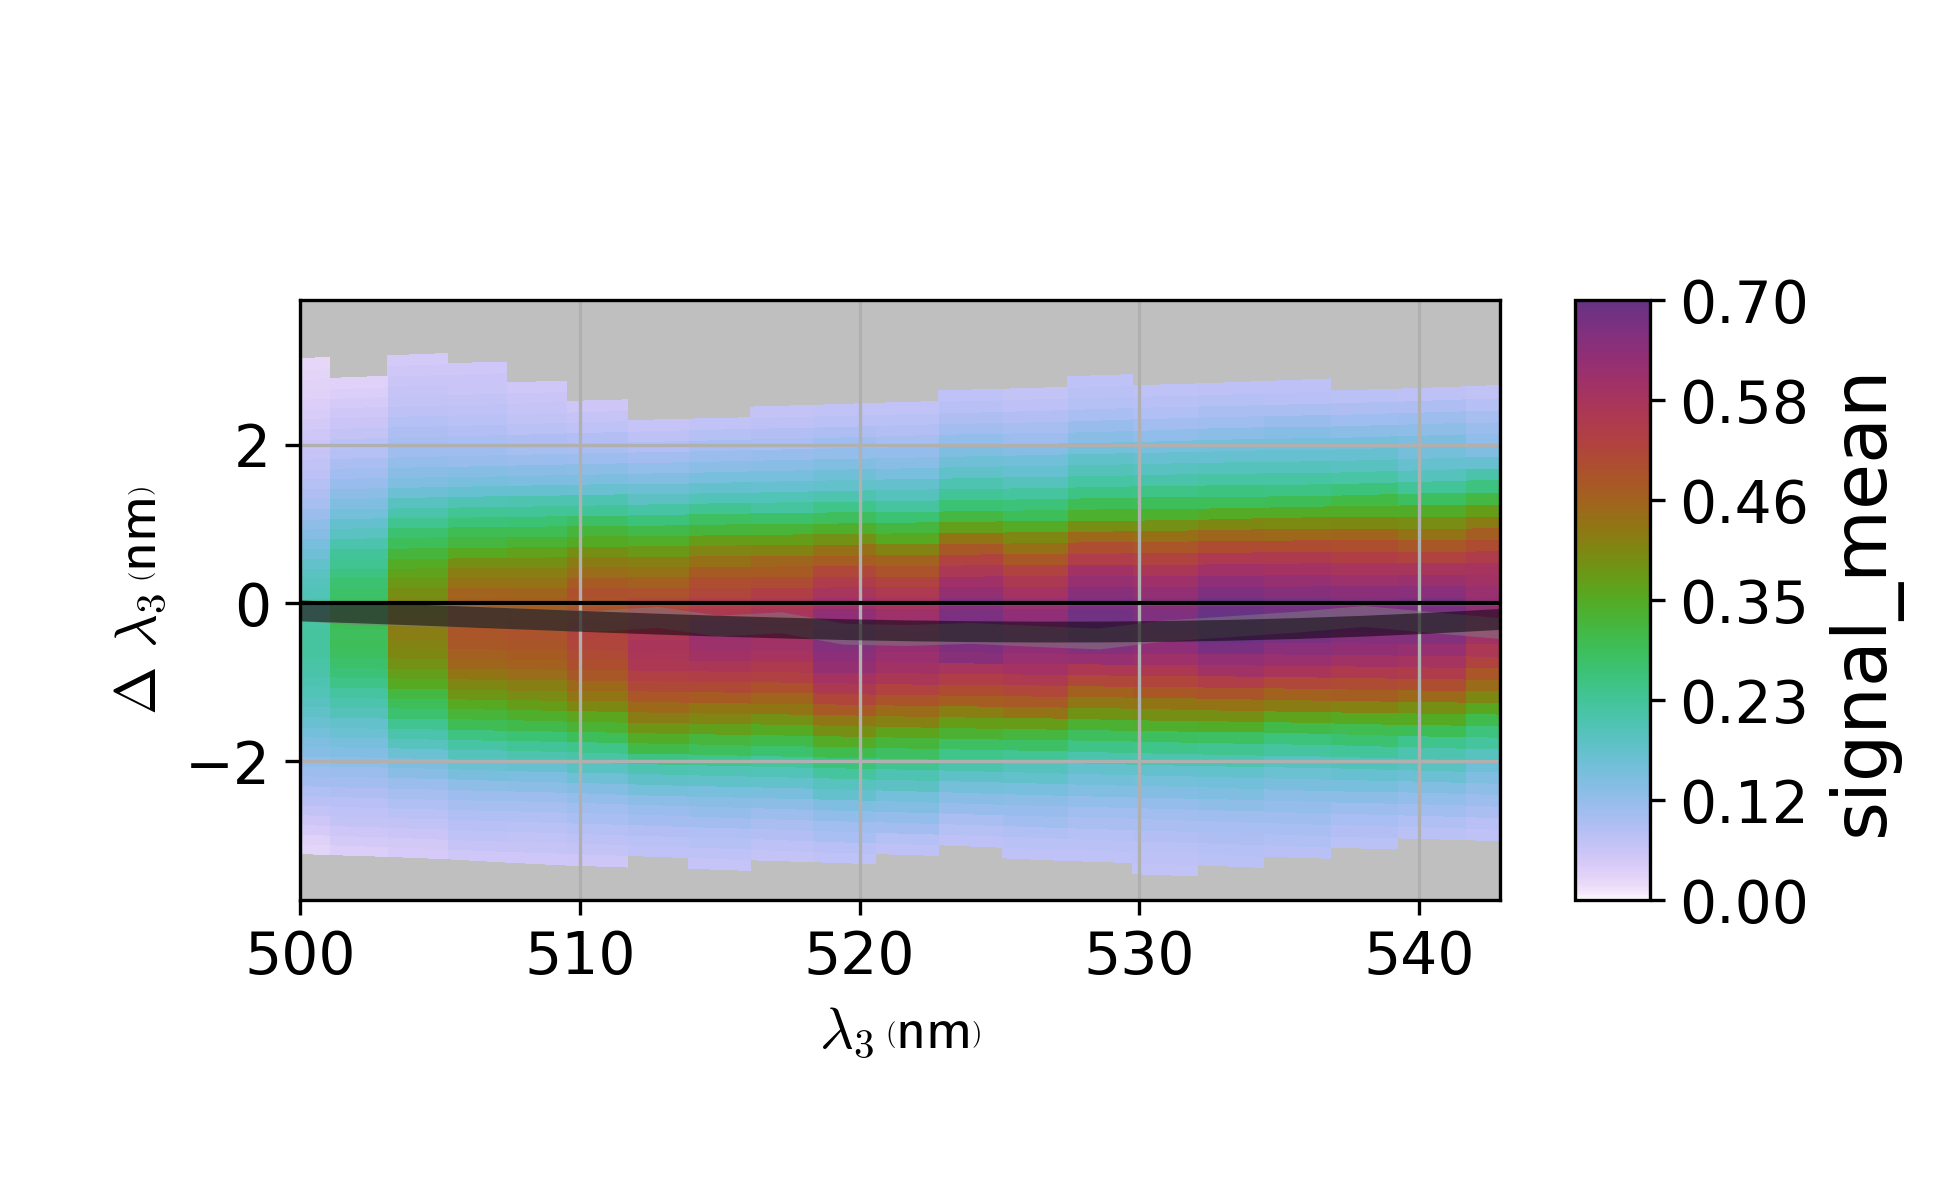
\includegraphics{representation/images/tune_test.png}
\caption[Tune Test]{
	An example plot created by \texttt{attune.tune\_test}.
}
\label{rep:fig:tune_test}
\end{figure}

The optimal tune test plot is flat at 0 deviation from expected color.

\hypertarget{intensity}{%
\subsubsection{intensity}\label{intensity}}

\texttt{attune.intensity} provides a mechanism to
update a single \texttt{attune.Tune} in an instrument
by optimizing the tune to provide the most intense position at each tune
point.

When passing an \texttt{attune.Instrument} to
\texttt{attune.intensity}, it is treated as updating
the existing position by adding to the existing positions. This is the
process when updating an OPA motor, which has been scanned as a
differential from the previous expected position against the opa tune
points. Any tunes other than the one specified as a parameter are
ignored and kept the same as the input
\texttt{attune.Instrument}. This method of tuning is
usually sufficient for OPAs in the picosecond regime, where pulse widths
allow each motor to be tuned independently. It is also used for later
motors in femtosecond tuning procedures such as the \texttt{delay\_2}
motor of a Light Conversion TOPAS-C OPA or any additional mixing process
after signal and idler have been generated.

Figure \ref{rep:fig:intensity} shows the plot associated with the following code:

\begin{codefragment}{python}
data.transform("w1=wm", "w1_Delay_2_points")
new = attune.intensity(
     data=data,
     channel=-1,
     arrangement="sig",
     tune="d2",
     instrument=old,
)
\end{codefragment}

\begin{figure}
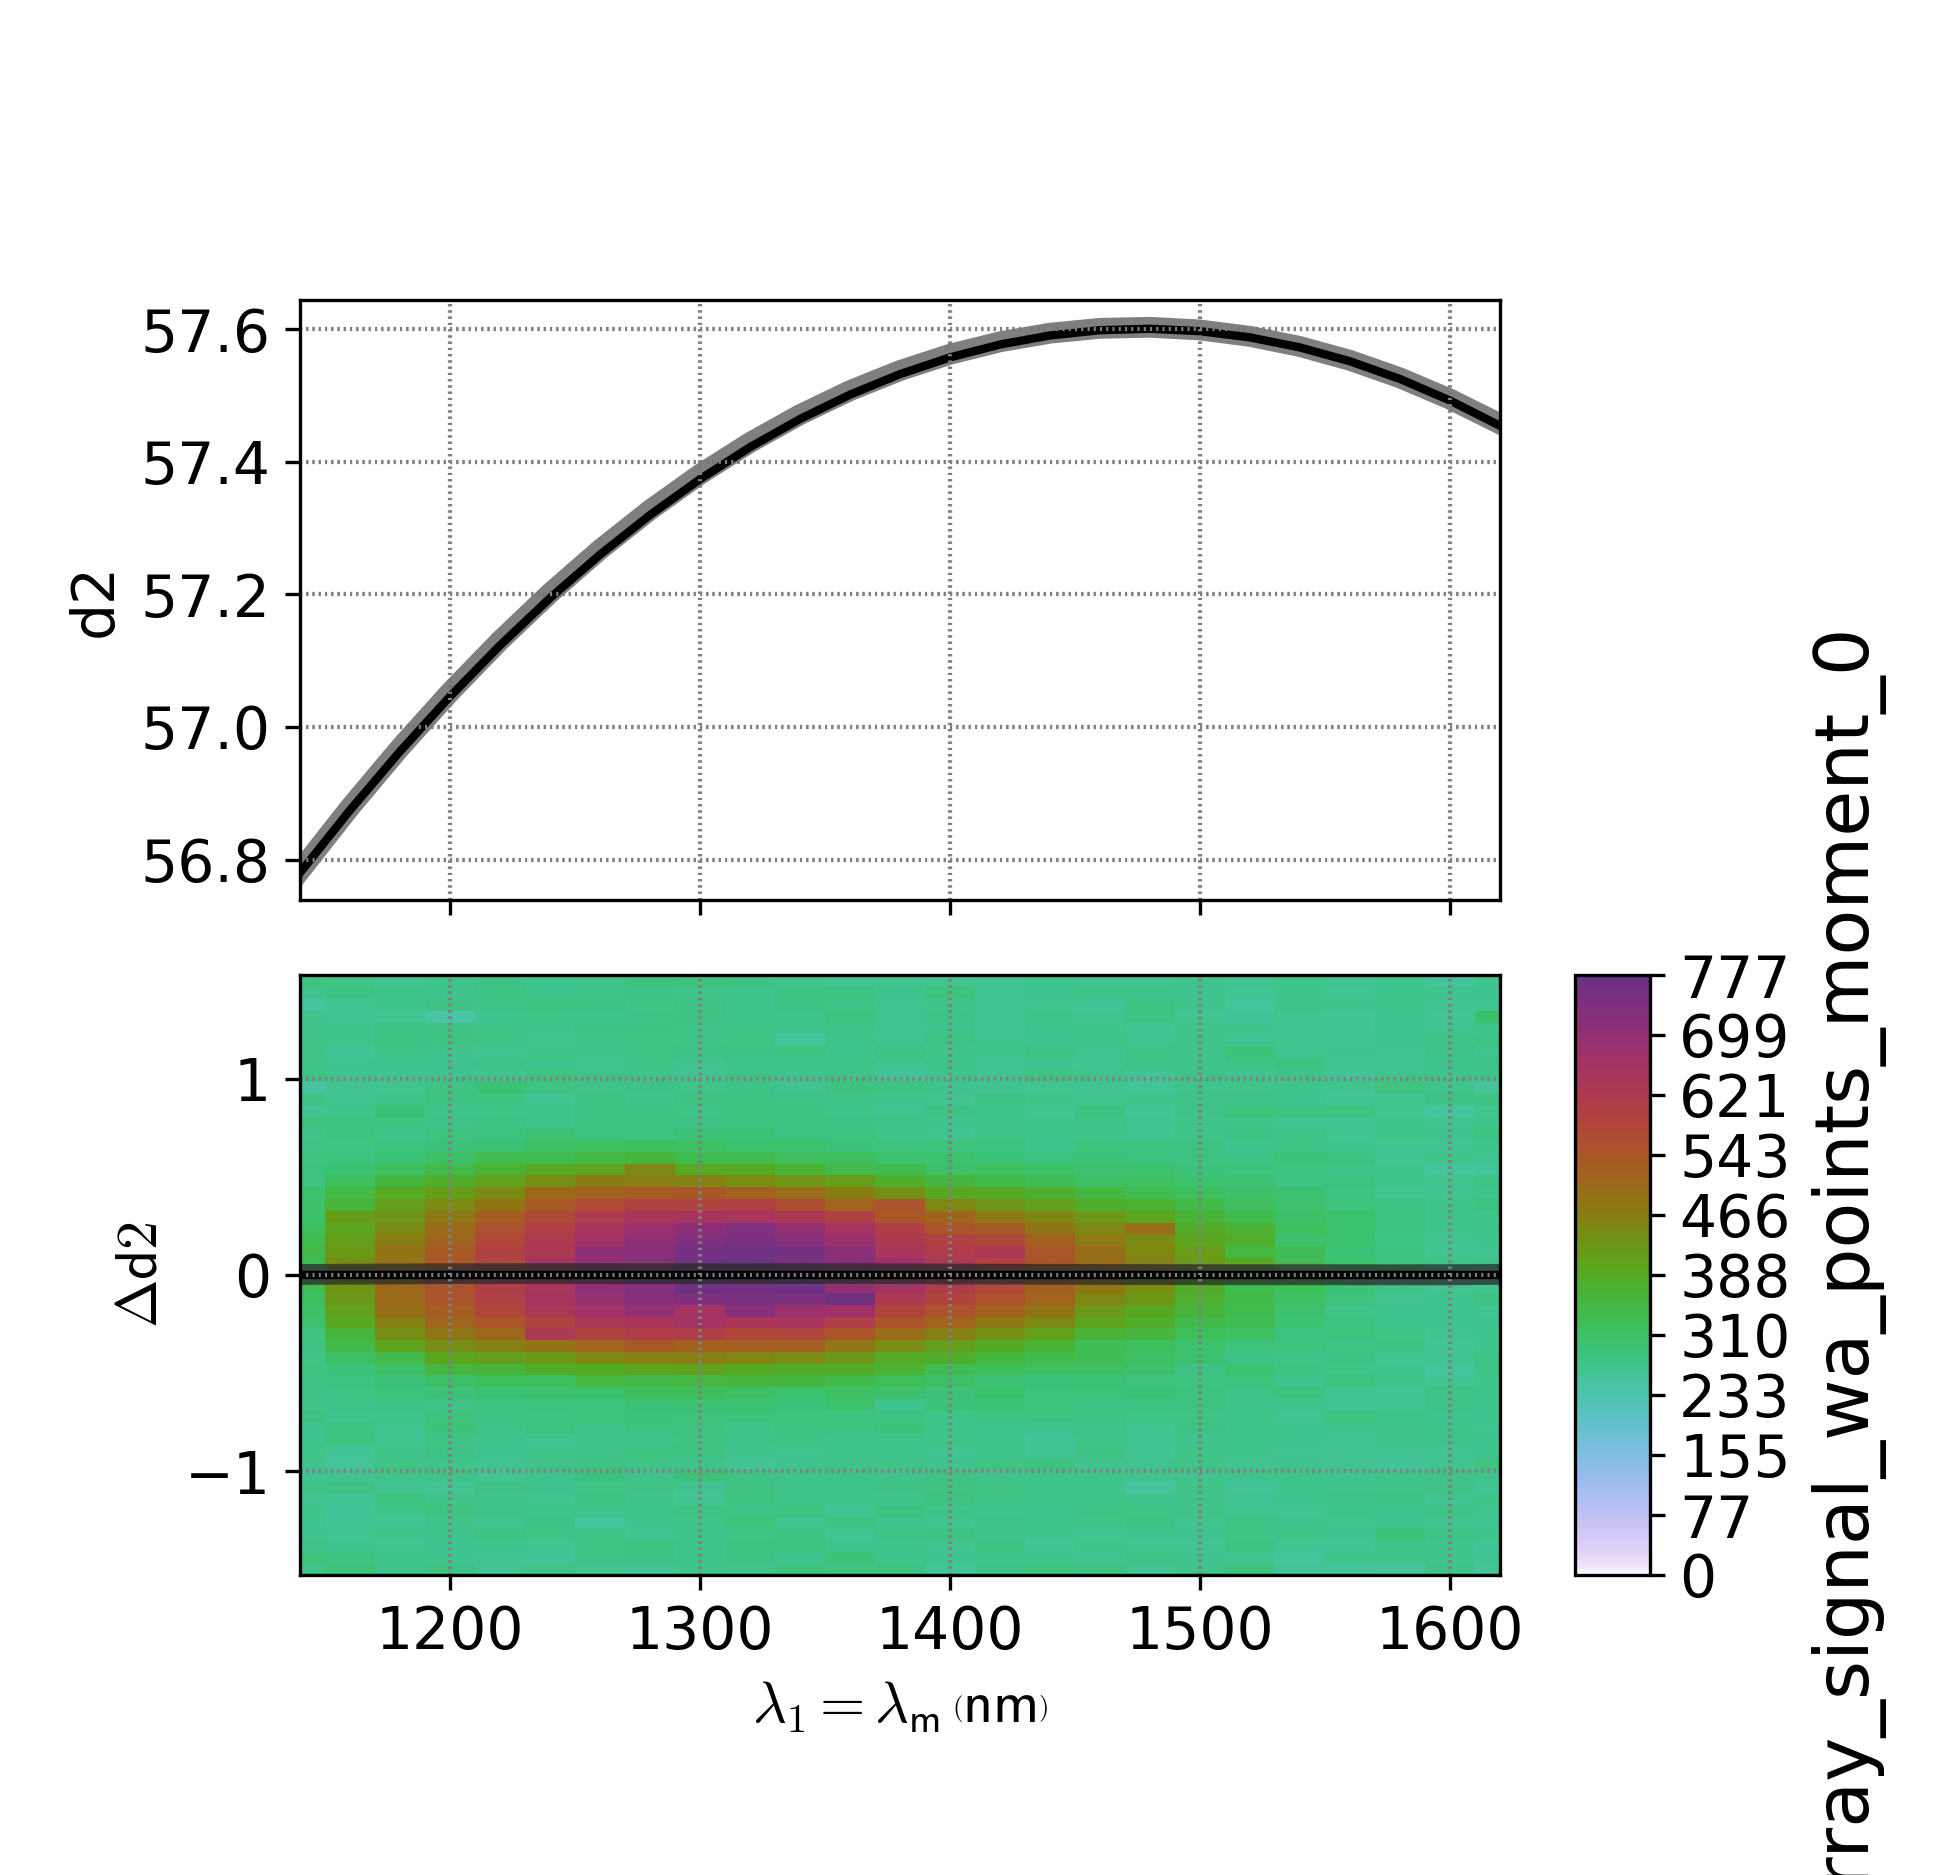
\includegraphics{representation/images/intensity.png}
\caption[Intensity]{
	An example plot created by \texttt{attune.intensity}.
}
\label{rep:fig:intensity}
\end{figure}

In the plot, the optimal position of the motor would be to follow the
ridge of the most intense peak.

When no \texttt{attune.Instrument} is provided,
\texttt{attune.intensity} creates a new
\texttt{attune.Instrument} containing only the one
tune. This is the process for generating a Spectral Delay Correction
\texttt{attune.Instrument} object. The scan for SDC is a delay position
(usually centered around 0) versus the OPA tune points. Since the output
instrument contains only a single arrangement with a single tune,
\texttt{attune.update\_merge} is often used to
recombine the SDC output into an instrument which contains SDC tunes for
alternate OPAs and arrangements of the same OPA.

\hypertarget{setpoint}{%
\subsubsection{setpoint}\label{setpoint}}

Instead of optimizing for output intensity,
\texttt{attune.setpoint} optimizes for the correctness
of the expected output color. This is useful for motors in femtosecond
OPAs which when perturbed change the overall intensity little, but
strongly affect the color produced, such as the Light Conversion TOPAS-C
\texttt{crystal\_2} motor.

The scan is nearly identical to the scan required for
\texttt{attune.intensity}, however since it is
optimising color information, a spectral axis (either via scanning a
monochromator or via an array detector) must be used. The data must be
transformed to (setpoint, differential\_motor\_position) The channel
must be pre-processed to contain the color information, rather than
intensity information. This is usually done by taking the
\texttt{WrightTools.data.Data.moment} with \texttt{moment=1} along the
spectral axis of the scan.

Figure \ref{rep:fig:setpoint} shows the plot associated with the following code:

\begin{codefragment}{python}
data.transform("w1=wm", "w1_Crystal_2_points", "wa-w1")
data.level(0, 2, 5)
data.array_signal.clip(min=0)
data.transform("w1=wm", "w1_Crystal_2_points", "wa")
data.moment("wa", moment=1, resultant=wt.kit.joint_shape(data.w1, data.w1_Crystal_2))
data.transform("w1=wm", "w1_Crystal_2_points")
data.channels[-1].clip(min=data.w1.min() - 1000, max=data.w1.max() + 1000)
data.channels[-1].null = data.wa.min()

out = attune.setpoint(
    data=data,
    channel=-1,
    arrangement="sig",
    tune="c2",
    instrument=instr,
)
\end{codefragment}

\begin{figure}
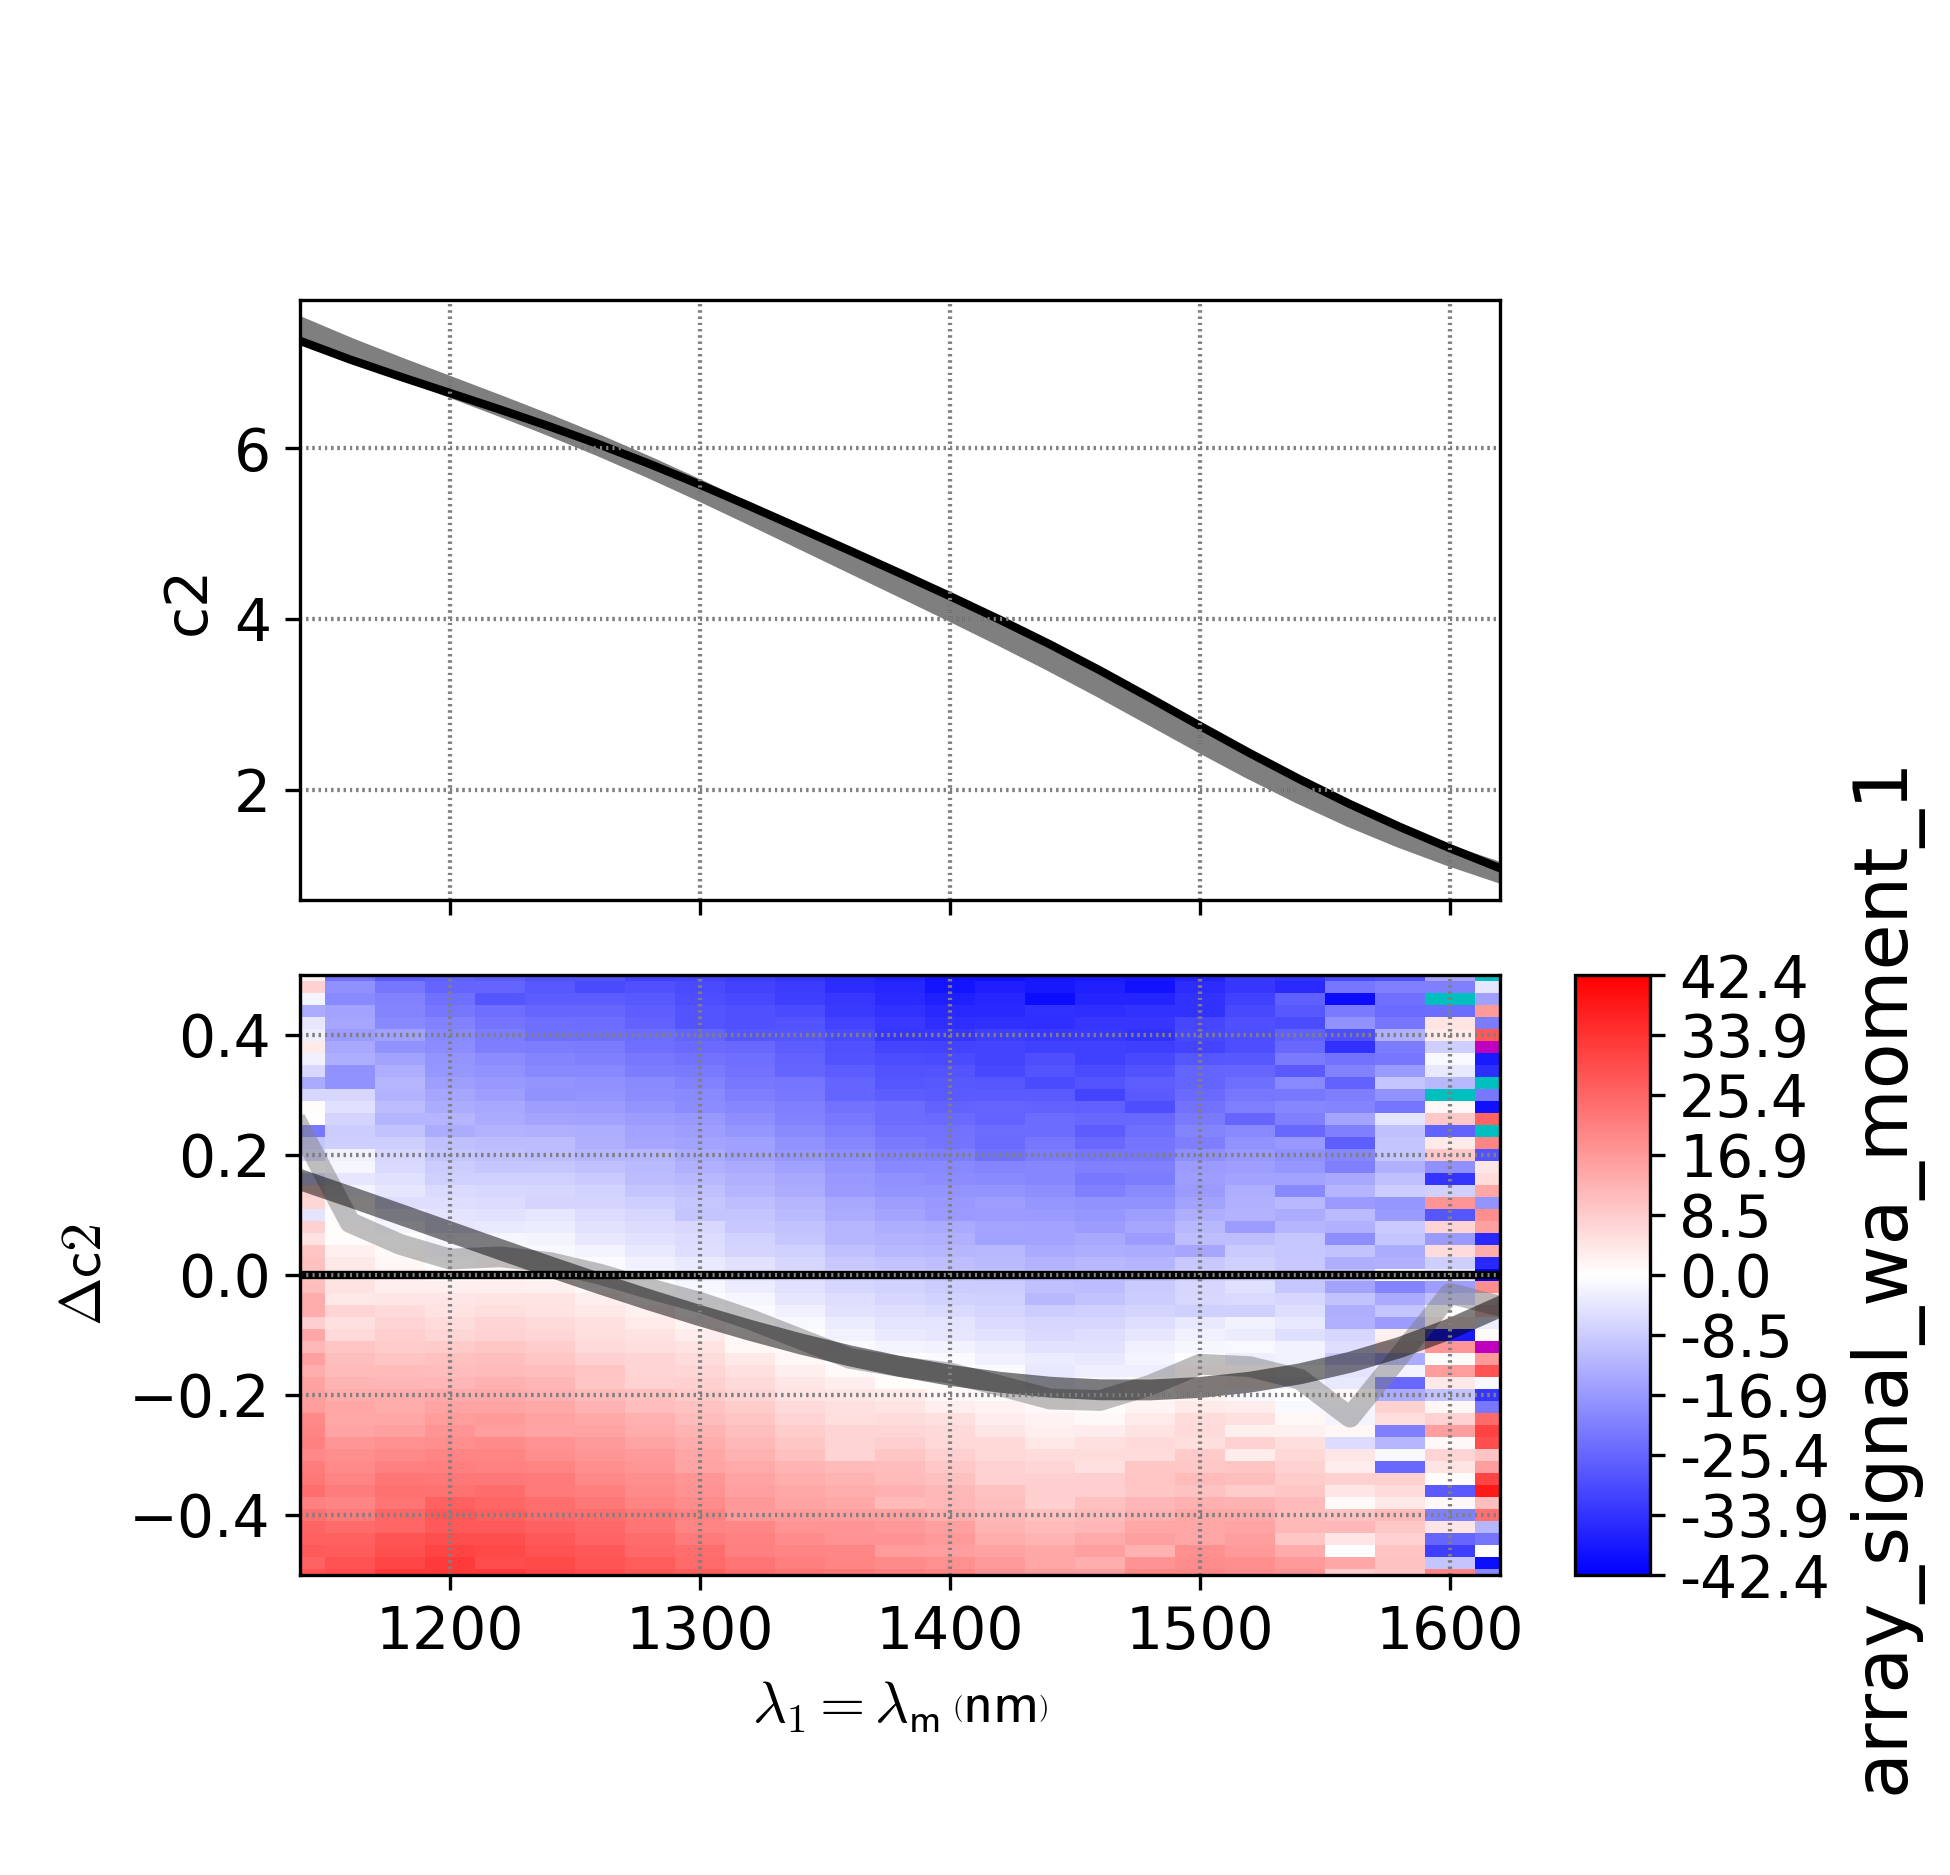
\includegraphics{representation/images/setpoint.png}
\caption[Setpoint]{
	An example plot created by \texttt{attune.setpoint}.
}
\label{rep:fig:setpoint}
\end{figure}

In the graph, the color represents deviation from the expected color and
pure white is the optimal motor position.

\hypertarget{holistic}{%
\subsubsection{holistic}\label{holistic}}

\texttt{attune.holistic} takes a multidimensional
approach by using both intensity and color information to optimize two
motors at once.

This is most useful for femtosecond OPAs where some motors are not
separable due to bandwidth of the pulse. As such for the Light
Conversion TOPAS-C OPAs, this is used to tune the "preamp" or
\texttt{crystal\_1} and \texttt{delay\_1}.

The scan for holistic actually looks very similar to the scan for
setpoint, including the OPA setpoint axis, a differential motor axis,
and a spectral axis (which could be from an array detector). However,
instead of being transformed to include the OPA setpoints, the transform
is applied such that \emph{two} motors are in the transform.

\texttt{attune.holistic} can either be handed separate
intensity and spectral channels (as a 2-tuple \texttt{channels}
argument) if separate preprocessing outside of the scope of the method
is required. In this case, it expects each channel to be two dimensional
and no spectral axis to be present in the channels or transform of the
data. If it is given a single channel it expects that the spectral axis
to be present and will take the 0th and 1st
\texttt{WrightTools.data.Data.moment} to get intensity and spectral
information, respectively) The spectral axis is assumed to be the last
axis of the transform as provide, but can be overridden using the
\texttt{spectral\_axes} parameter.

The algorithm for \texttt{attune.holistic} starts by
clipping data below the \texttt{gtol} for the amplitude channel,
applying the clip to both the amplitude and color channels (as you
cannot get a reliable color estimate from values below the noise
threshold). It then creates a
\texttt{scipy.interpolate.LinearNDInterpolator} for each of the
amplitude and spectral channels. It finds the point on each edge of the
\texttt{scipy.spatial.Delaunay} interpolation triangles which are the
color of each tune point. If enough points are found that are the
requested color, it fits the points to a Gaussian function using the
intensity information, one Gaussian for each dimension. It then splines
each motor against the input color, and replaces the tunes in the input
instrument with the new splined positions.

In principle, this algorithm generalizes to an arbitrary number of
dimensions, however the plotting step in particular only works for 2
dimensional data.

Figure \ref{rep:fig:holistic} shows the plot associated with the following code:

\begin{codefragment}{python}
data.transform("w1_Crystal_1", "w1_Delay_1", "wa")
out = attune.holistic(
    data=data,
    channels="array_signal",
    arrangement="NON-NON-NON-Sig",
    tunes=["c1", "d1"],
    instrument=instr,
    gtol=0.05,
    level=True,
)
\end{codefragment}

\begin{figure}
	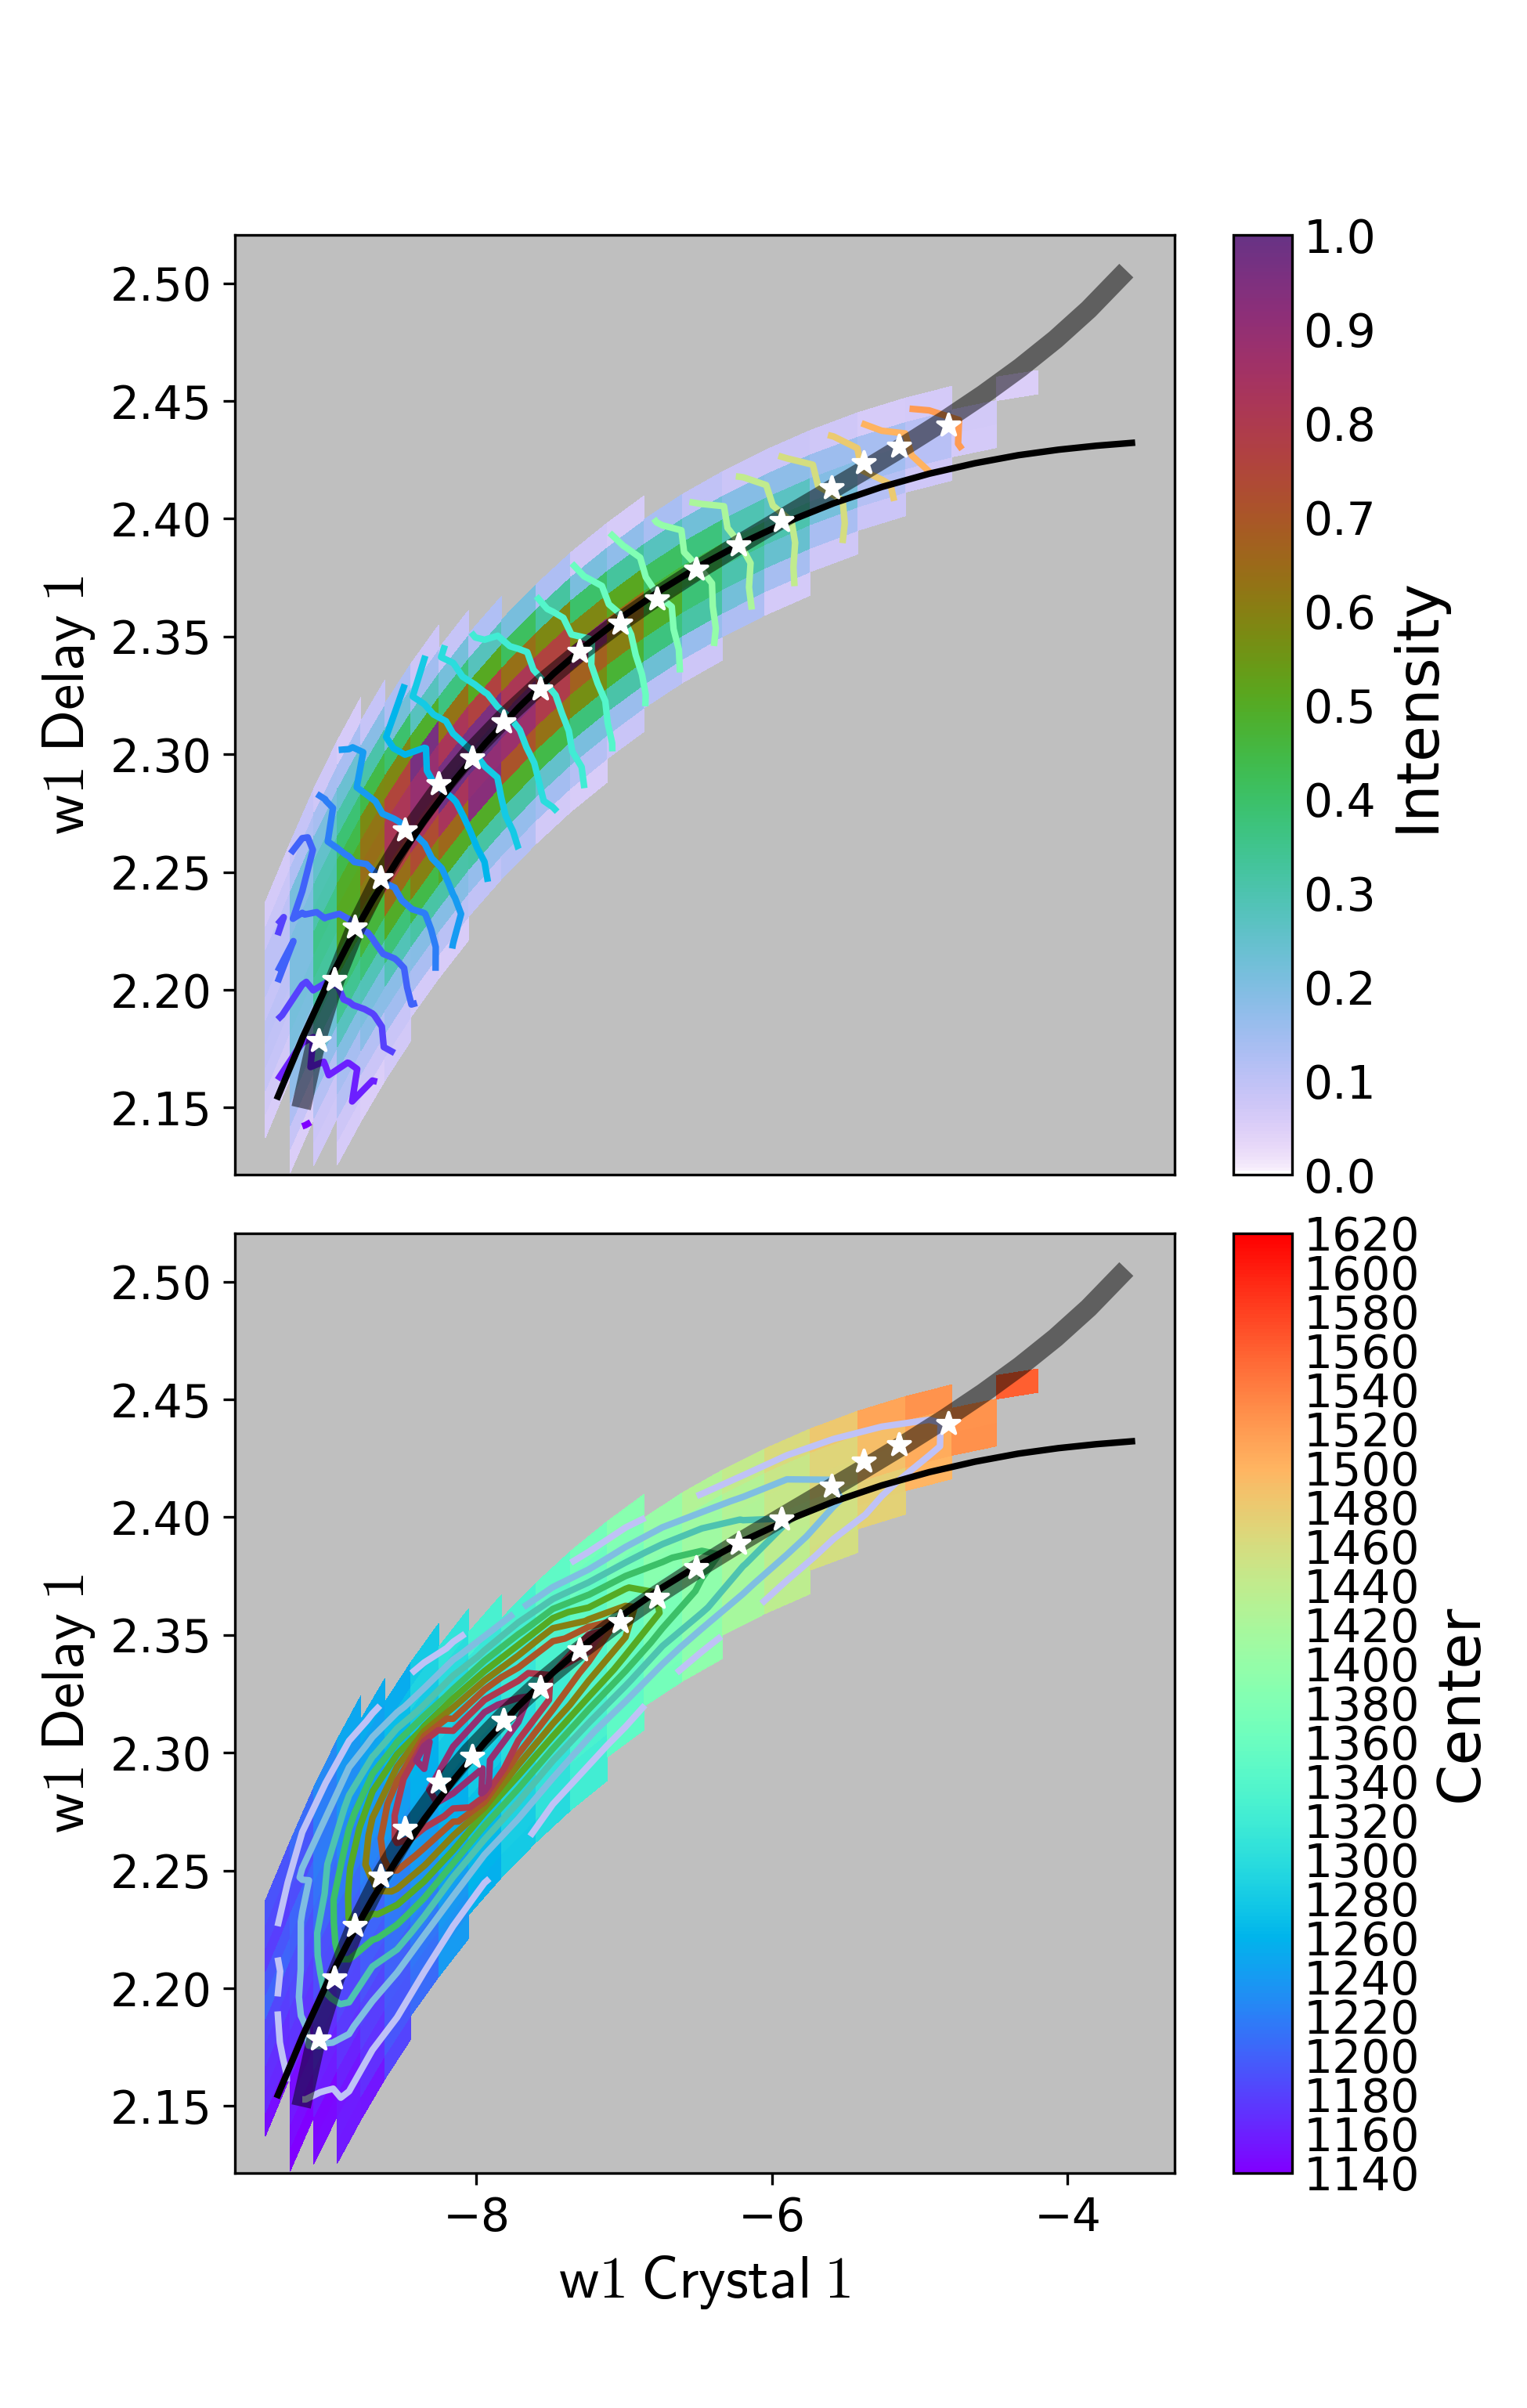
\includegraphics[width=5in]{representation/images/holistic.png}
\caption[Holistic]{
	An example plot created by \texttt{attune.holistic}.
}
\label{rep:fig:holistic}
\end{figure}

The axes of both plots are in 2D motor-space. The top plot is an
intensity plot with contours of constant color overlaid. The bottom plot
is the inverse: color plot with contours of constant intensity overlaid.
The thin black line is the input path through 2D motor space. The thick
semitransparent line is the output selected path through 2D motor space.
The stars are the points which were selected by the algorithm for each
tune point. Ideally, the thick black line would be along the ridge of
the "slug" shape.

\clearpage
